\documentclass[machines,article,submit,moreauthors]{Definitions/mdpi}
\graphicspath{{../papers/figures/}}
\setlength{\headheight}{20pt}
% Suppress the MDPI template's unassigned, metadata-derived DOI in submit mode.
\AtBeginDocument{%
  \rfoot{}%
  \fancypagestyle{plain}{\rfoot{}}%
}
\firstpage{1}
\makeatletter
\setcounter{page}{\@firstpage}
\makeatother
\pubvolume{1}
\issuenum{1}
\articlenumber{0}
\pubyear{2026}
\copyrightyear{2026}
\Title{A Dual-Mode Electrohydraulic Hitch Control Architecture for Long-Term Position Holding in Agricultural Machinery: A Parameterized Virtual-Prototype Stress Test}
\newcommand{\orcidauthorA}{0009-0005-1928-6218}
\Author{Chenyu Cui$^{1}$, Peng Wang$^{1}$ and Yucheng Zhang$^{1,}$*\orcidA{}}
\AuthorNames{Chenyu Cui, Peng Wang and Yucheng Zhang}
\address{%
$^{1}$ \quad Prospective Research Laboratory, Institute of Computing Technology, Chinese Academy of Sciences, Beijing 100190, China}
\corres{Correspondence: zhangyucheng@ict.ac.cn}
\datereceived{}
\daterevised{}
\dateaccepted{}
\datepublished{}
\abstract{Long-duration position holding is a machinery-control requirement for electrohydraulic three-point hitches because a small retained loss can become a large implement-position error during operation. This study develops a dual-mode electrohydraulic control architecture for a heavy agricultural-machinery hitch and evaluates it in a reproducible, parameterized virtual prototype. The model evolves a reduced pressure-difference state, reconstructs paired virtual pressure outputs for controller access, and includes command saturation, friction, temperature-dependent virtual leakage, position noise, a lock-mode loss path, and an accumulator charging/discharge branch. A known-input pressure-transition residual updates a model-level leakage coefficient. During tracking, a boundary-layer sliding-mode controller is combined with pressure feedforward. After the reference is reached, a hysteretic supervisor selects bounded valve trimming, locking, or accumulator compensation; load feedforward updates the holding-pressure target. Twenty seeded simulations were performed for an 1800 s hold, alongside a declared one-at-a-time assumption-range screen and a 32-case Cartesian interaction surface. Under a filtered-velocity entry criterion, the complete controller had a full-run root-mean-square error of 9.24 mm and a mean hold drop of 0.022 mm. In a 14 kN load-step test, accumulator closed-loop compensation and load feedforward reduced mean drop from 20.85 mm and 96.59 mm, respectively, to 1.75 mm. All 640 Cartesian virtual runs passed a predeclared 10 mm, 1800 s drop screen. A separate controller-facing measurement audit retained the failure of unfiltered 0.1 MPa pressure noise and found an 8.97 mm worst steady error for a declared combined mismatch with 0.05 MPa noise and a 200 ms pressure filter. These results quantify architecture-level behavior and internal consistency for a machine-control design screen, not physical-machine performance. The unfiltered velocity gate did not enter hold in the present simulations, and the hydraulic inputs are declared virtual-model definitions rather than target-machine measurements.}
\keyword{agricultural machinery; electrohydraulic actuator; three-point hitch; position control; virtual prototype; stress testing; supervisory control}
\begin{document}

\section{Introduction}
Rear hitches must accomplish two tasks with fundamentally different time scales: move an implement to a commanded position and maintain that position after motion has ended. Position holding is not merely the final portion of a tracking transient. It governs implement-depth retention, hydraulic energy consumption, and valve activity while the tractor operates under a quasi-static load. During this phase, cylinder and lock-valve leakage, load changes, temperature, sensor noise, and the available hydraulic storage can all produce a slow position drift. A controller optimized only for tracking can therefore generate unnecessary valve activity or fail to distinguish a persistent loss path from a transient disturbance.

The practical importance of this distinction is increasing as tractor hitches are integrated with automated depth control and coordinated traction functions. A recent review of tractor electrohydraulic hitch systems documents the breadth of position, draft, and mixed-control architectures used in agricultural machinery \cite{sun2022}. At the component level, the flow characteristics of a tractor electrohydraulic hitch valve have been modelled and experimentally validated \cite{kumar2021}; at the system level, coordinated hitch-depth and travel-speed control has been studied as an efficiency-oriented agricultural operation \cite{sun2025}. These studies motivate a clear representation of the hydraulic and supervisory mechanisms that govern a transition from commanded motion to holding.

Recent tractor research has also reported hitch-position estimation using an EKF--Transformer architecture \cite{kim2025} and robust draft/position control with differential and integral sliding modes \cite{liu2023}. More generally, electrohydraulic servo research provides established sliding-mode and adaptive-control designs \cite{bai2010,tang2011,jin2013}. These contributions establish useful control ingredients, but their performance evidence has different objectives from a long-hold stress test: many studies emphasize trajectory tracking, draft regulation, or a specific hardware configuration rather than the entry logic, retained leakage path, and storage-assisted response during an extended hold.

For a holding study, the evaluation protocol must also be separated from the eventual acceptance claim. A small average drop can arise because a controller has not entered its hold mode, because the disturbance is unrealistically smooth, or because an internal pressure state is available without sensor error. Conversely, a conservative velocity gate can prevent a nominally stable controller from being evaluated at all. Reporting the entry criterion, time horizon, load disturbance, and parameter range is therefore as important as reporting a single position error. This distinction is especially important for a theoretical model, where repeatable seeded noise provides an internal stress test but cannot substitute for independent trials on a hydraulic machine.

This work therefore investigates a narrow, simulation-based question: can a leakage-informed state supervisor coordinate tracking, bounded valve trim, locking, and accumulator compensation under explicitly stated assumptions? The goal is not to estimate the field performance of a particular hitch. Instead, the virtual prototype makes its loss paths, internal pressure access, parameter classes, and stress conditions inspectable so that a reviewer can distinguish internal model consistency from physical validation.

\section{Related Work}
Prior work on tractor hitches can be grouped into system development, agricultural-operation coordination, and electrohydraulic servo control. System-development studies describe the sensing, hydraulic, and control choices required for electrohydraulic hitches \cite{sun2022}, while component studies such as the valve-flow analysis of Kumar et al. \cite{kumar2021} provide physically useful evidence for a specific valve. Coordinated depth and speed control addresses a different but complementary agricultural objective: it connects the hitch command to operation quality and economy \cite{sun2025}. None of these results makes a calibrated hydraulic data set available for the virtual prototype studied here, so they are used to position the problem rather than to identify its numerical parameters.

In electrohydraulic motion control, reduced servo models are commonly used to expose the coupling among pressure, valve flow, load, and position before a specific machine is identified \cite{jelali2003}. Sliding-mode and adaptive methods then manage nonlinearities and disturbances \cite{bai2010,tang2011,jin2013}. Tractor-specific work similarly combines draft and position objectives \cite{liu2023}, and estimator-based work can improve the availability of hitch-position information \cite{kim2025}. However, a conventional tracking comparison does not directly test whether a controller should trim, lock, or draw from a hydraulic accumulator once the reference is reached. That decision depends on the assumed retained loss and on the entry criterion for the hold state.

The present study contributes at this supervisory level. It separates cylinder and lock-path losses in a reduced-order model, exposes a pressure-transition residual as a model-level leakage proxy, and reports both a filtered entry result and the failure of the original raw-velocity gate. The resulting evidence is deliberately limited to a parameterized virtual prototype. It supplies an auditable long-duration stress-test workflow, not a claim that the described policy has been calibrated or validated on a physical tractor.

For a machinery and mechatronics readership, the architectural contribution is the explicit separation of motion control, hold-state supervision, and stored-fluid compensation. This separation makes the actuator interfaces and failure-sensitive transitions visible: a reviewer can inspect which branch is active, which pressure signal is assumed available, and how a load step is absorbed. The study therefore treats the virtual prototype as a design-screening instrument for an electrohydraulic machine, with the same distinction between model-consistency evidence and hardware validation retained throughout the paper.

\section{Materials and Methods}
\subsection{Electrohydraulic hitch model}
The plant is a reduced-order pressure-difference virtual surrogate, not a two-chamber fluid-conservation model. Let $x$, $v$, and $d$ denote piston position, velocity, and virtual pressure difference. At each explicit 10 ms step, the implementation evaluates
\begin{equation}
 d_{k+1}=\Pi_{[0,p_{\mathrm{rel}}]}\left[d_k+\Delta t\left\{a_m(d_k^\star-d_k)-g_m\mathcal{L}(d_k,T_k;C_l,g_T)+\frac{\beta_e}{V}q_{\mathrm{acc},k}\right\}\right],
\end{equation}
where $d_k^\star=(F_{L,k}+kx_k+F_f)/A+G_p\operatorname{sat}_{[-1,1]}(u_k)$. The mode coefficient $a_m$ is $a_{\mathrm{track}}$ or $a_{\mathrm{hold}}$; $g_m$ is one in tracking and the declared retained-loss term in hold. $\mathcal{L}$ is the implementation-defined virtual loss operator, with its scalar $C_l$ multiplied linearly above 25 $^\circ$C by $g_T$. The accumulator term is zero outside accumulator-assisted hold. Thus, $G_p$, $a_m$, $g_m$, and $g_T$ are explicitly reduced-order coefficients, rather than valve or fluid data-sheet parameters. The mechanical state is updated by
\begin{equation}
 m\dot v=Ad-F_L-cv-F_f(v)-kx,\qquad \dot x=v.
\end{equation}
For controller interfaces only, paired virtual pressure outputs are reconstructed from $d$ and a bounded common pressure; they are not separately conserved chamber states. Nominal runs expose the noise-free virtual pressure difference, while the independent observability audit supplies controller-facing position, pressure, and load perturbations without changing the plant. This distinction makes the nominal pressure interface an explicit virtual-model assumption rather than a sensor-performance claim.

An accumulator is represented by a precharge pressure, gas volume, discharge valve, and recharge branch. Its discharge flow is
\begin{equation}
q_{acc}=u_{acc}K_{acc}\max(p_{acc}-d,0),\qquad
p_{acc}=\max\left(1.01d,\;p_{acc,0}\frac{V_{acc,0}}{V_{acc,0}+V_{out}}\right).
\end{equation}
This is a virtual compensation branch with a bounded recharge proxy. It is not a calibrated representation of a particular accumulator, lock valve, or hydraulic circuit.

\subsection{Parameter provenance and assumption register}
All 22 plant parameters used by the reported virtual prototype are listed in the machine-readable file \texttt{paper1\_parameter\_manifest.csv}. Each row has a stable identifier, code identifier, numerical value, unit, source class, model role, and stress-test coverage. The companion assumption register records the scope and prohibited physical interpretation of each modelling choice. The file \texttt{export\_paper1\_traceability.py} checks every manifest value against \texttt{LiftParameters}, snapshots the experiment and controller defaults, and exports SHA-256 fingerprints before reproduction. Table~\ref{tab:provenance} summarizes the source classes. No value is represented as a manufacturer data-sheet value or a calibrated physical measurement.

\begin{table}[H]
\centering
\caption{Traceable parameter source classes for the paper-1 virtual prototype.}
\label{tab:provenance}
\resizebox{\textwidth}{!}{%
\begin{tabular}{lcl}
\toprule
Source class & Count & Interpretation \\
\midrule
Virtual hydraulic input & 9 & Researcher-defined virtual cylinder, loss, pressure-limit, and accumulator inputs \\
Virtual mechanical input & 5 & Researcher-defined inertia, friction, stiffness, and stroke inputs \\
Reduced-order coefficient & 6 & Command-to-pressure, mode-relaxation, thermal, and pressure-reconstruction settings \\
Numerical setting & 1 & Explicit integration interval \\
Measurement setting & 1 & Seeded position-noise standard deviation \\
\bottomrule
\end{tabular}
}
\end{table}

\subsection{Assumption ranges and stress screens}
Table~\ref{tab:assumptions} lists selected values with dedicated stress screens. Except for position noise, the listed ranges are deterministic one-at-a-time settings rather than estimated probability distributions. They test whether the conclusions are locally fragile within the virtual model; they do not quantify uncertainty of a physical hitch.

\begin{table}[H]
\centering
\caption{Selected virtual-prototype inputs and one-at-a-time stress settings. Full provenance and all nominal values are in \texttt{paper1\_parameter\_manifest.csv}; none is an identified physical measurement.}
\label{tab:assumptions}
\resizebox{\textwidth}{!}{%
\begin{tabular}{llll}
\toprule
Quantity & Nominal value & Stress settings & Role in model \\
\midrule
Moving mass $m$ & 1200 kg & $0.7m$, $1.3m$ & actuator inertia \\
Viscous coefficient $c$ & 2200 N s m$^{-1}$ & $0.7c$, $1.3c$ & mechanical damping \\
Hitch stiffness $k$ & 18 000 N m$^{-1}$ & $0.7k$, $1.3k$ & load-position relation \\
Cylinder leakage $C_l$ & $1.5\times10^{-12}$ m$^3$ s$^{-1}$ Pa$^{-1}$ & $0.5C_l$, $2C_l$, $5C_l$ & pressure loss \\
Position-noise SD & 1.5 mm & 0.5, 2.0$\times$ & measured position \\
Accumulator flow coefficient & $2.0\times10^{-12}$ m$^3$ s$^{-1}$ Pa$^{-1}$ & 0.5, 1.5$\times$ at 14 kN & compensation branch \\
\bottomrule
\end{tabular}
}
\end{table}

\subsection{Control architecture}
Figure~\ref{fig:architecture} shows the architecture. During the commanded motion, the controller combines a pressure-balance feedforward term with PID, DI-SMAC, or boundary-layer sliding-mode feedback. When the accumulator is inactive, the known command and load define a leakage-free pressure-rate prediction $\dot{\Delta p}^{(0)}_k$. The pressure-transition residual gives a non-negative coefficient candidate,
\begin{equation}
 C^*_{l,k}=\frac{A\max\{a_m(d_k^\star-d_k)-(d_{k+1}-d_k)/\Delta t,0\}}{g_m d_k[1+g_T\max(T_k-25,0)]},
\end{equation}
where $g_m=1$ in tracking and $g_m=0.08(1-u_{comp})$ in hold. The proxy applies an exponential update $\hat C_{l,k+1}=(1-\alpha)\hat C_{l,k}+\alpha C^*_{l,k}$ with $\alpha=0.08$ and does not update while the accumulator is discharging, because its virtual flow would confound a leakage-only residual. This is a model inversion diagnostic, not a physical leakage-identification method.

The hold supervisor is entered only after the position error is within 10 mm and the velocity gate is satisfied for 1 s. It applies hysteresis between fine trim, lock, and accumulator modes. The holding pressure target uses the measured or estimated implement load. Accumulator mode is selected by either the leakage-flow threshold or a measured pressure deficit above 0.08 MPa, so that a load step can invoke stored-fluid support without being misclassified as a leakage event. When the accumulator mode is active, its discharge valve is driven by pressure deficit and a bounded position-error integral; the main valve remains in bounded fine trim. For the observability audit, the pressure interface can apply a declared first-order measurement filter; its time constant is part of the evaluated controller interface, not a plant calibration. This separation avoids the opposing main-valve/accumulator actions observed in an earlier implementation.

\begin{figure}[H]
\centering
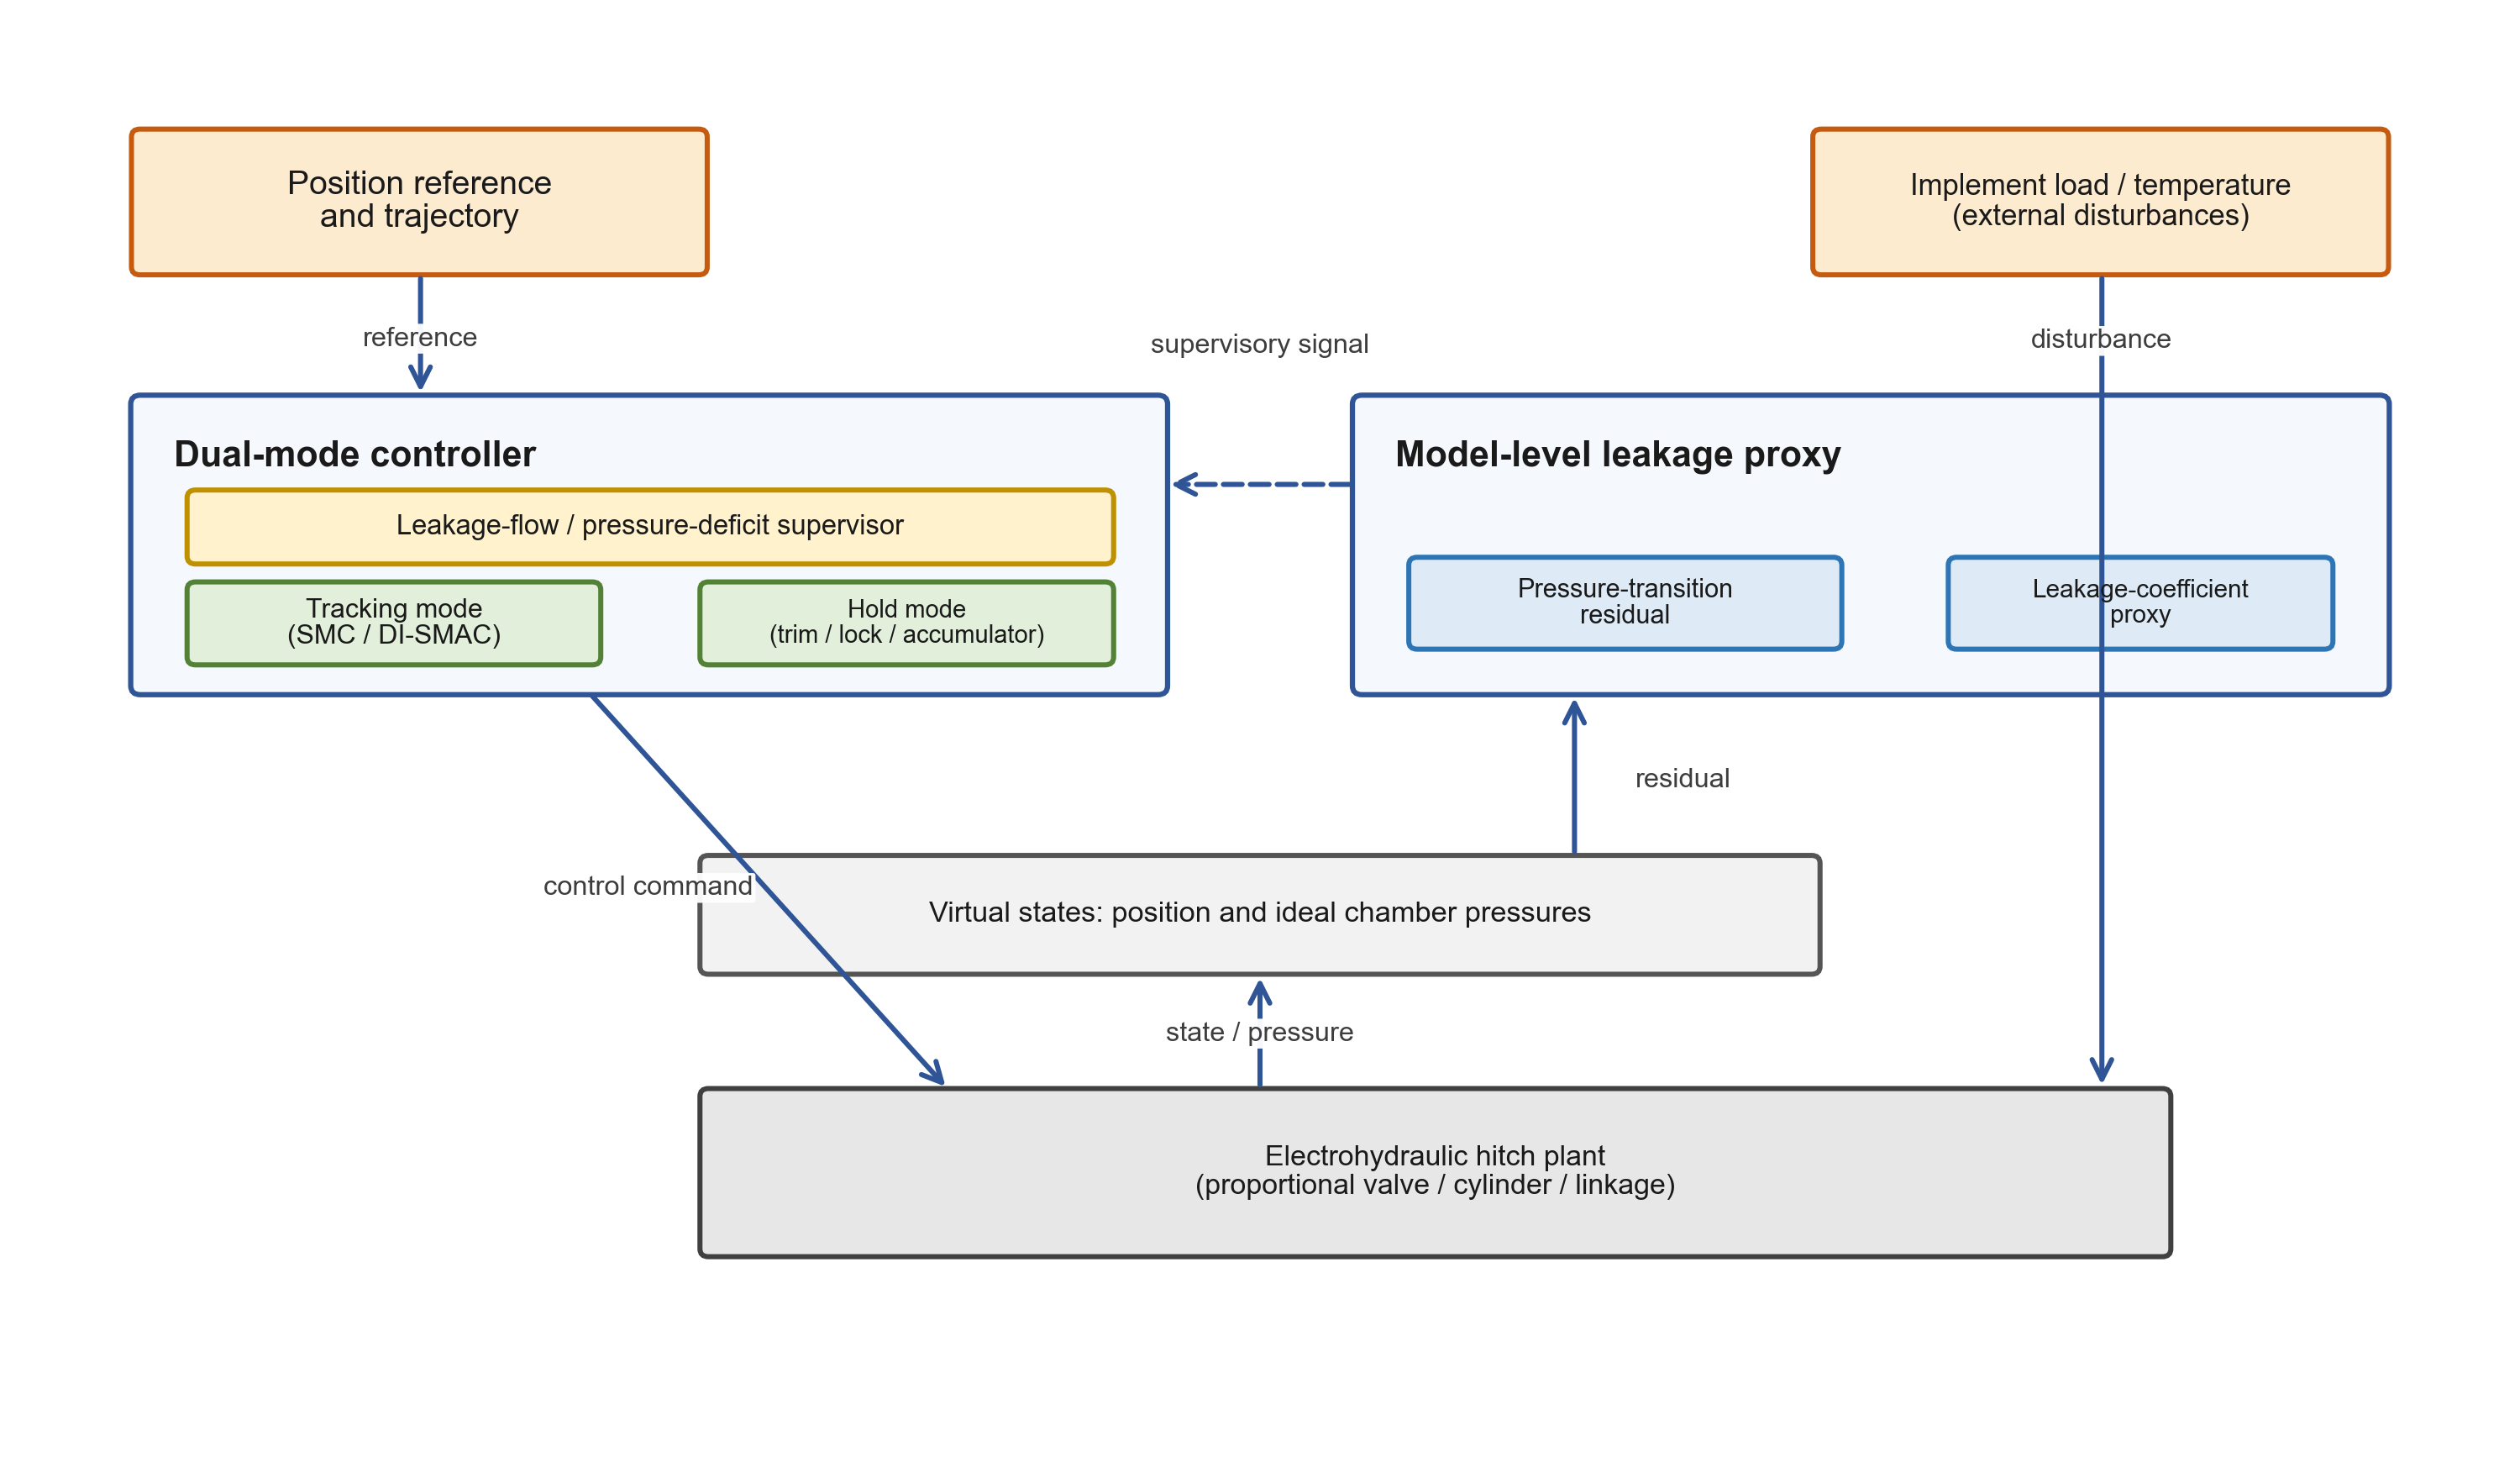
\includegraphics[width=0.96\linewidth]{paper1_architecture.png}
\caption{Dual-mode hitch-control architecture with a model-level pressure-transition leakage proxy.}
\label{fig:architecture}
\end{figure}

\subsection{Boundedness argument}
The analysis assumes bounded load and leakage-rate variation, bounded inversion error, a bounded valve command, and operation below the relief-pressure limit. For a bounded candidate error $\epsilon_k=C^*_{l,k}-C_l$, the observation error $\tilde C_l=C_l-\hat C_l$ obeys
\begin{equation}
|\tilde C_{l,k+1}|\le(1-\alpha)|\tilde C_{l,k}|+\alpha\bar\epsilon.
\end{equation}
Thus, for $0<\alpha<1$, the proxy is ultimately bounded by the virtual-model inversion error. This is not a robust hardware theorem under arbitrary pressure-sensor, valve, or accumulator errors. The separate measurement audit only quantifies selected controller-facing perturbations and retains its unfiltered-noise failure boundary. For the sliding variable $s=\lambda(x_r-x)+v$, the boundary-layer controller gives a negative drift outside the boundary layer when the switching gain exceeds the disturbance and noise bounds. Finally, if residual hold leakage is bounded by $\bar q_l$, a conservative screening condition is
\begin{equation}
\Delta x_{1800}\le \frac{1800\bar q_l}{A}+\Delta x_{valve}+\Delta x_{structure}.
\label{eq:drop}
\end{equation}
Equation~\eqref{eq:drop} is a parameterized criterion, not proof of a physical-hardware requirement.

\subsection{Simulation protocol and statistics}
The virtual prototype was simulated at 10 ms for 1800 s. Position followed a smooth 0.15 m to 0.35 m reference over 8 s. The load was 9 kN for the first 10 s and 7 kN afterwards; oil temperature rose from 25 to 40 $^\circ$C; position-noise standard deviation was 1.5 mm. Twenty seeds (2026--2045) were used for the primary, temperature-load, and leakage-step protocols. The one-at-a-time range screen used five fixed seeds (2026--2030), because it is a deterministic assumption check rather than a field-trial estimator. The complete hybrid controller was compared with anti-windup PID, DI-SMAC, and boundary-layer SMC; all methods used the same plant, reference, noise sequence, and common hold supervisor. This shared-supervisor comparison is an ablation of the tracking branch, not an end-to-end ranking of independently designed hold controllers.

The outcome metrics were full-run RMSE, terminal position error, hold-entry time, 1800 s position drop, command energy, and hold-entry rate. The filtered velocity gate, raw velocity gate, and their conjunction were evaluated separately. Ablations removed load feedforward, accumulator closed-loop compensation, the leakage proxy, hysteresis, or the hold structure. A 14 kN step, leakage multipliers, and a 60 s cylinder-leakage step from one to eight times nominal were used as virtual stress tests.

\section{Results}
\subsection{Nominal tracking and holding}
Table~\ref{tab:main} gives the 20-seed results under the filtered-velocity definition. The controllers have similar RMSE because they share the pressure feedforward and hold supervisor. The approximately 200 mm dynamic maximum error is the initial 0.20 m commanded displacement and must not be interpreted as steady-state tracking error. The hybrid controller had 4.27 mm terminal error and 0.022 mm mean hold drop.

\begin{table}[H]
\centering
\caption{Results for the parameterized 1800 s test (mean $\pm$ standard deviation, $n=20$). Hold-entry rate uses the filtered velocity gate.}
\label{tab:main}
\resizebox{\textwidth}{!}{%
\begin{tabular}{lrrrrr}
\toprule
Controller & RMSE (mm) & Terminal error (mm) & Hold entry (s) & Hold drop (mm) & Entry rate \\
\midrule
PID & $9.179\pm0.004$ & $4.138\pm0.253$ & $8.207\pm0.116$ & $0.017\pm0.021$ & 100\% \\
DI-SMAC & $9.233\pm0.008$ & $4.288\pm0.277$ & $8.464\pm0.190$ & $0.019\pm0.023$ & 100\% \\
Boundary-layer SMC & $9.228\pm0.005$ & $4.254\pm0.266$ & $8.503\pm0.181$ & $0.014\pm0.020$ & 100\% \\
Dual-mode hybrid & $9.236\pm0.006$ & $4.267\pm0.296$ & $8.523\pm0.157$ & $0.022\pm0.027$ & 100\% \\
\bottomrule
\end{tabular}
}
\end{table}

The raw-velocity and dual-gate definitions produced zero hold entries in all 20 runs. This is a material result: filter delay is part of the present hold-entry behavior, so the filtered result cannot be treated as a direct safety statement for a real hitch.

\subsection{Leakage and load-step stress tests}
Figure~\ref{fig:leak} shows the lock-valve leakage-path sensitivity. The mean drop remained below 0.088 mm at ten times the assumed lock-path leakage. This margin only describes the low-leakage parameterization. It cannot replace temperature-dependent lock-valve measurements.

\begin{figure}[H]
\centering
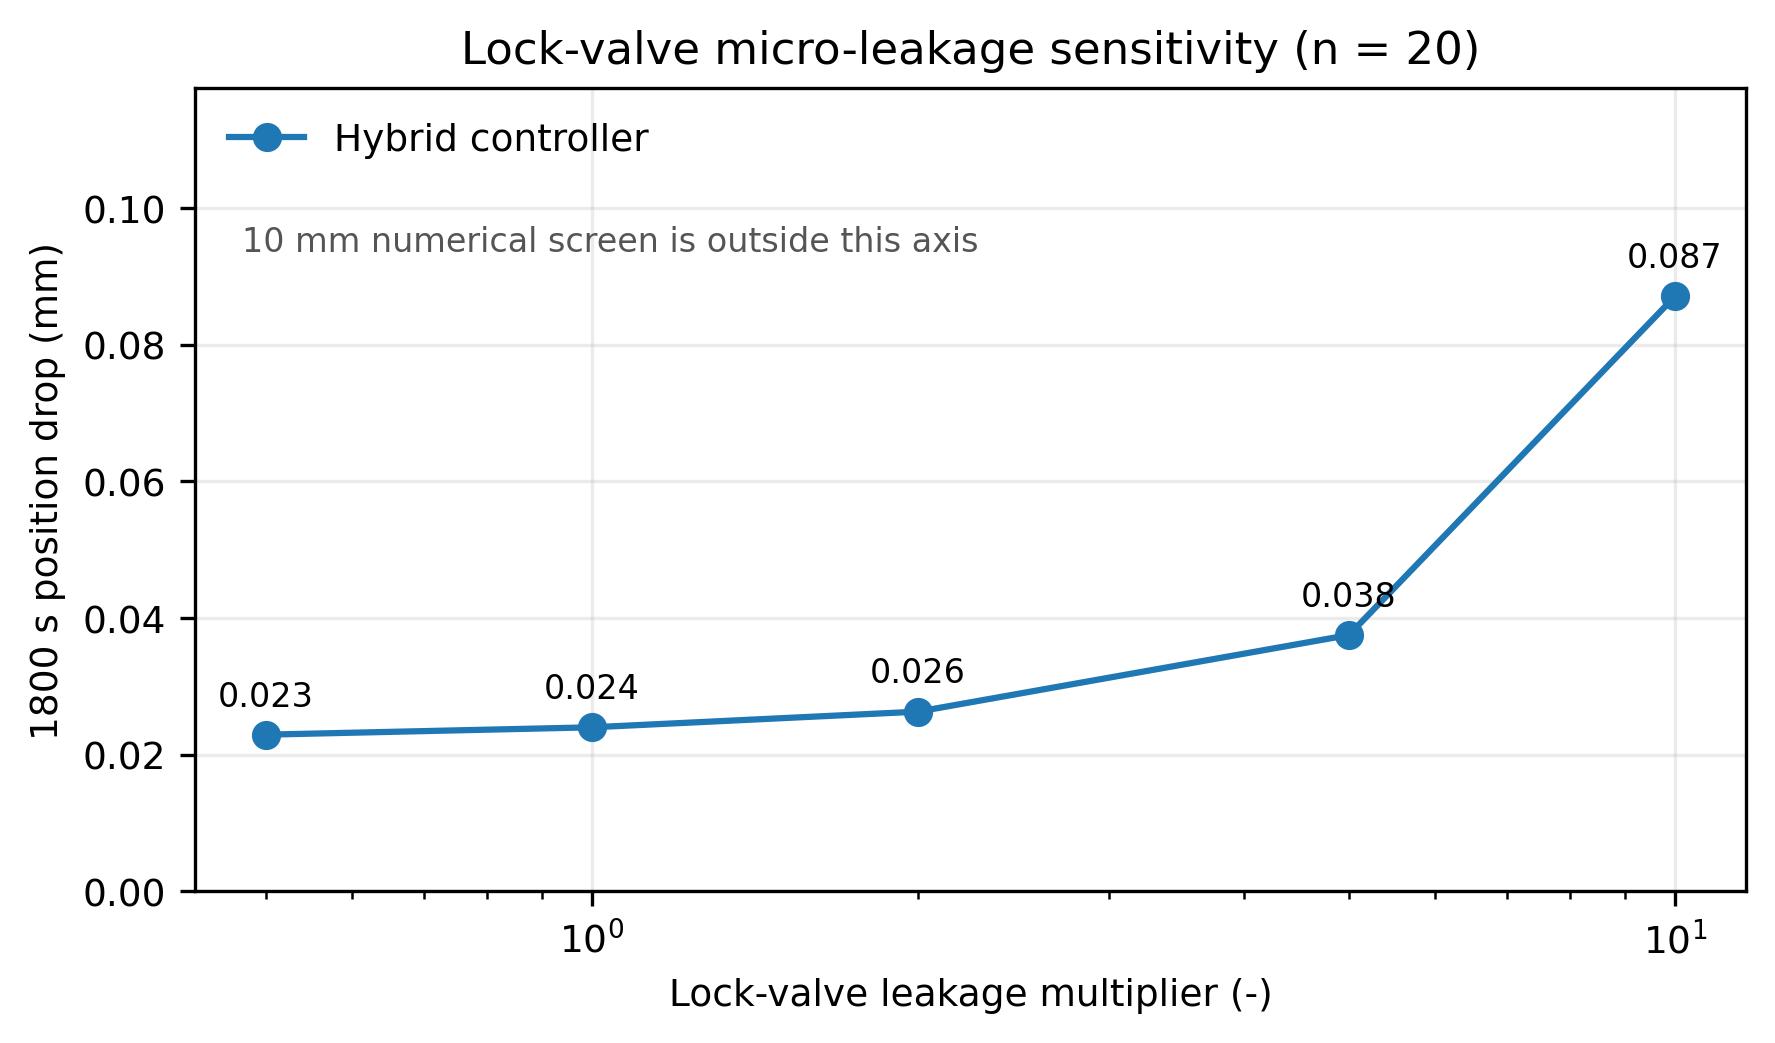
\includegraphics[width=0.76\linewidth]{paper1_lock_leakage_sensitivity.png}
\caption{Sensitivity of the complete controller to the assumed lock-valve micro-leakage path ($n=20$).}
\label{fig:leak}
\end{figure}

The more discriminating ablation is the 14 kN load step (Figure~\ref{fig:ablation}). With load feedforward and accumulator closed-loop compensation, the mean drop was 1.75 mm. Removing the accumulator closed loop increased it to 20.85 mm, and removing load feedforward increased it to 96.59 mm. The results show that the claimed benefit is conditional on a correct load signal, the modeled pressure-deficit trigger, and available accumulator pressure.

\begin{figure}[H]
\centering
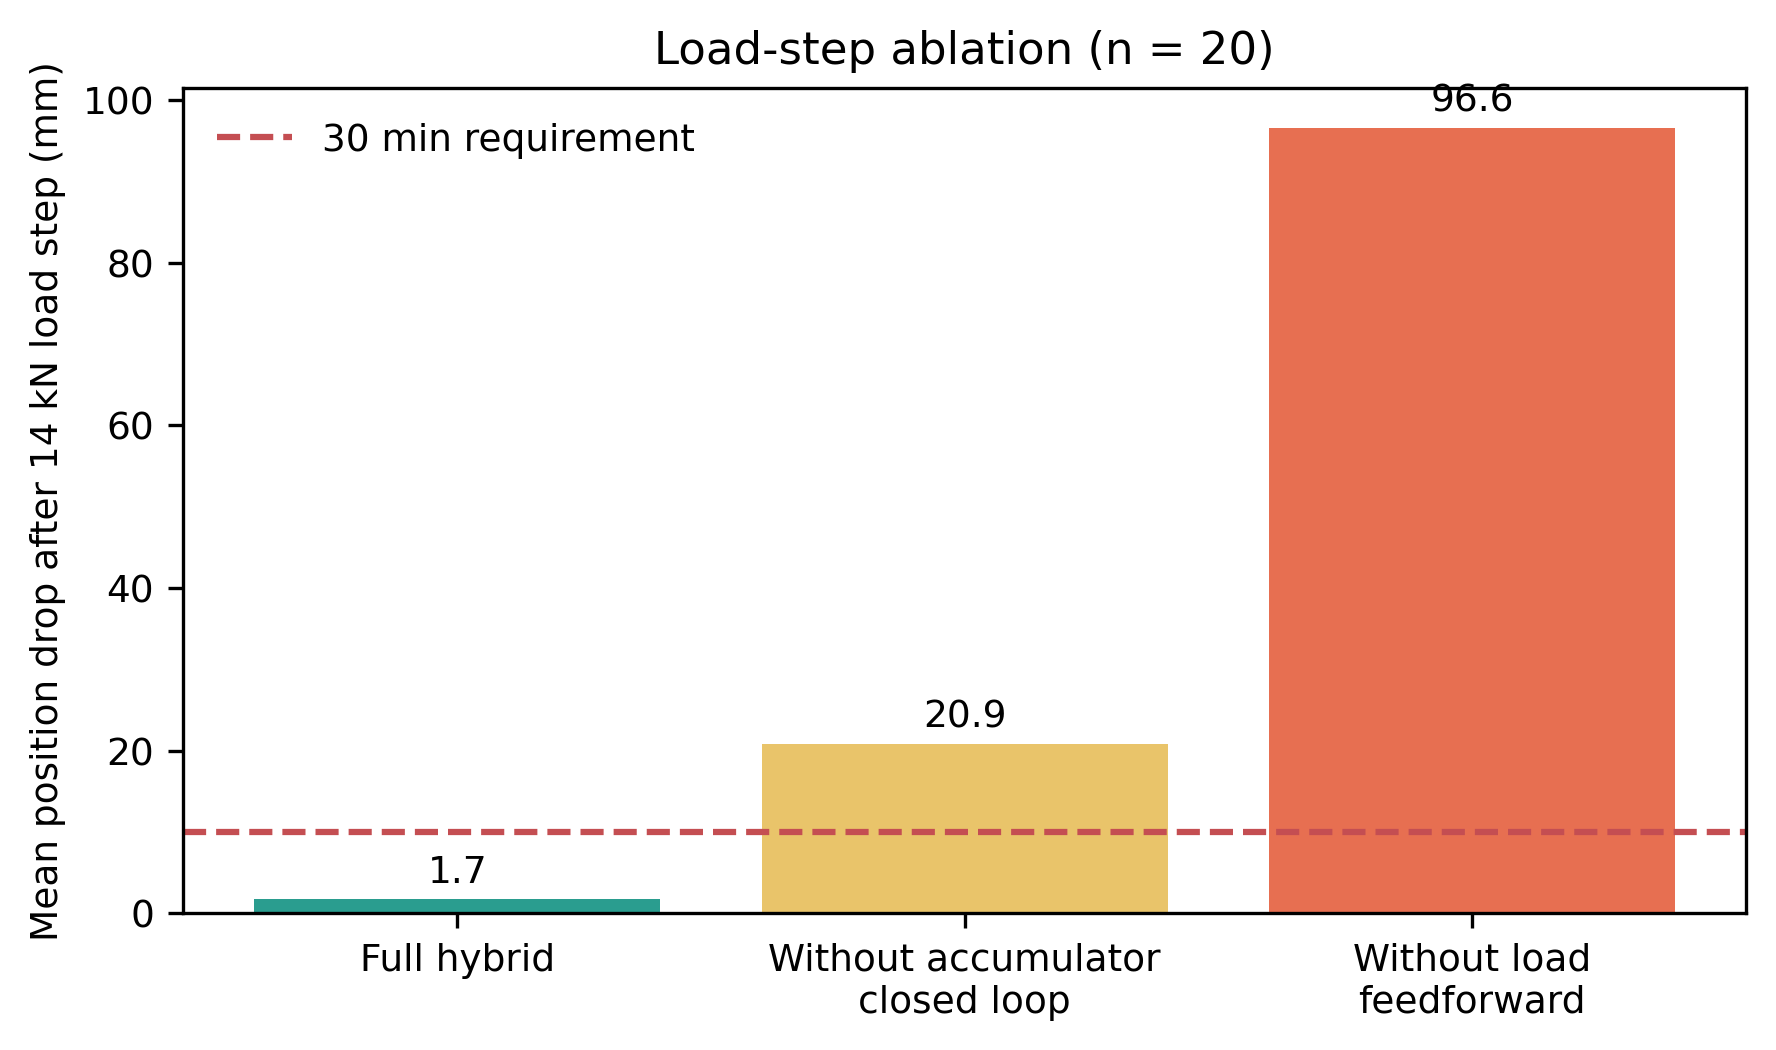
\includegraphics[width=0.76\linewidth]{paper1_load_step_ablation.png}
\caption{Load-step ablation for a 14 kN step. The dashed line is the assumed 10 mm, 30 min requirement ($n=20$).}
\label{fig:ablation}
\end{figure}

\subsection{Assumption-range and virtual leakage-step screens}
Figure~\ref{fig:assumption-proxy} summarizes selected one-at-a-time stress settings. Across the mass, damping, stiffness, position-noise, and cylinder-leakage settings in Table~\ref{tab:assumptions}, all five-seed cases entered hold and their mean 1800 s drop was below 0.060 mm. At the 14 kN step, the assumed accumulator-flow coefficient was consequential: 0.5$\times$ and 1.5$\times$ its nominal value gave mean drops of 5.86 mm and 0.273 mm, respectively. These are model-structure sensitivities, not confidence bounds on a real hydraulic circuit.

For a virtual cylinder-leakage step at 60 s from one to eight times the nominal coefficient, the pressure-transition proxy reached 90\% of the new coefficient in $0.255\pm0.005$ s ($n=20$) and ended at $1.200\times10^{-11}$ m$^3$ s$^{-1}$ Pa$^{-1}$; a fixed nominal prior remained at $1.5\times10^{-12}$ m$^3$ s$^{-1}$ Pa$^{-1}$. Both cases entered hold in 20/20 runs and had the same 0.022 mm mean drop. Thus, the test demonstrates internal state-transition and supervisory-mode consistency, not an independent position-holding advantage or physical leakage identification.

\begin{figure}[H]
\centering
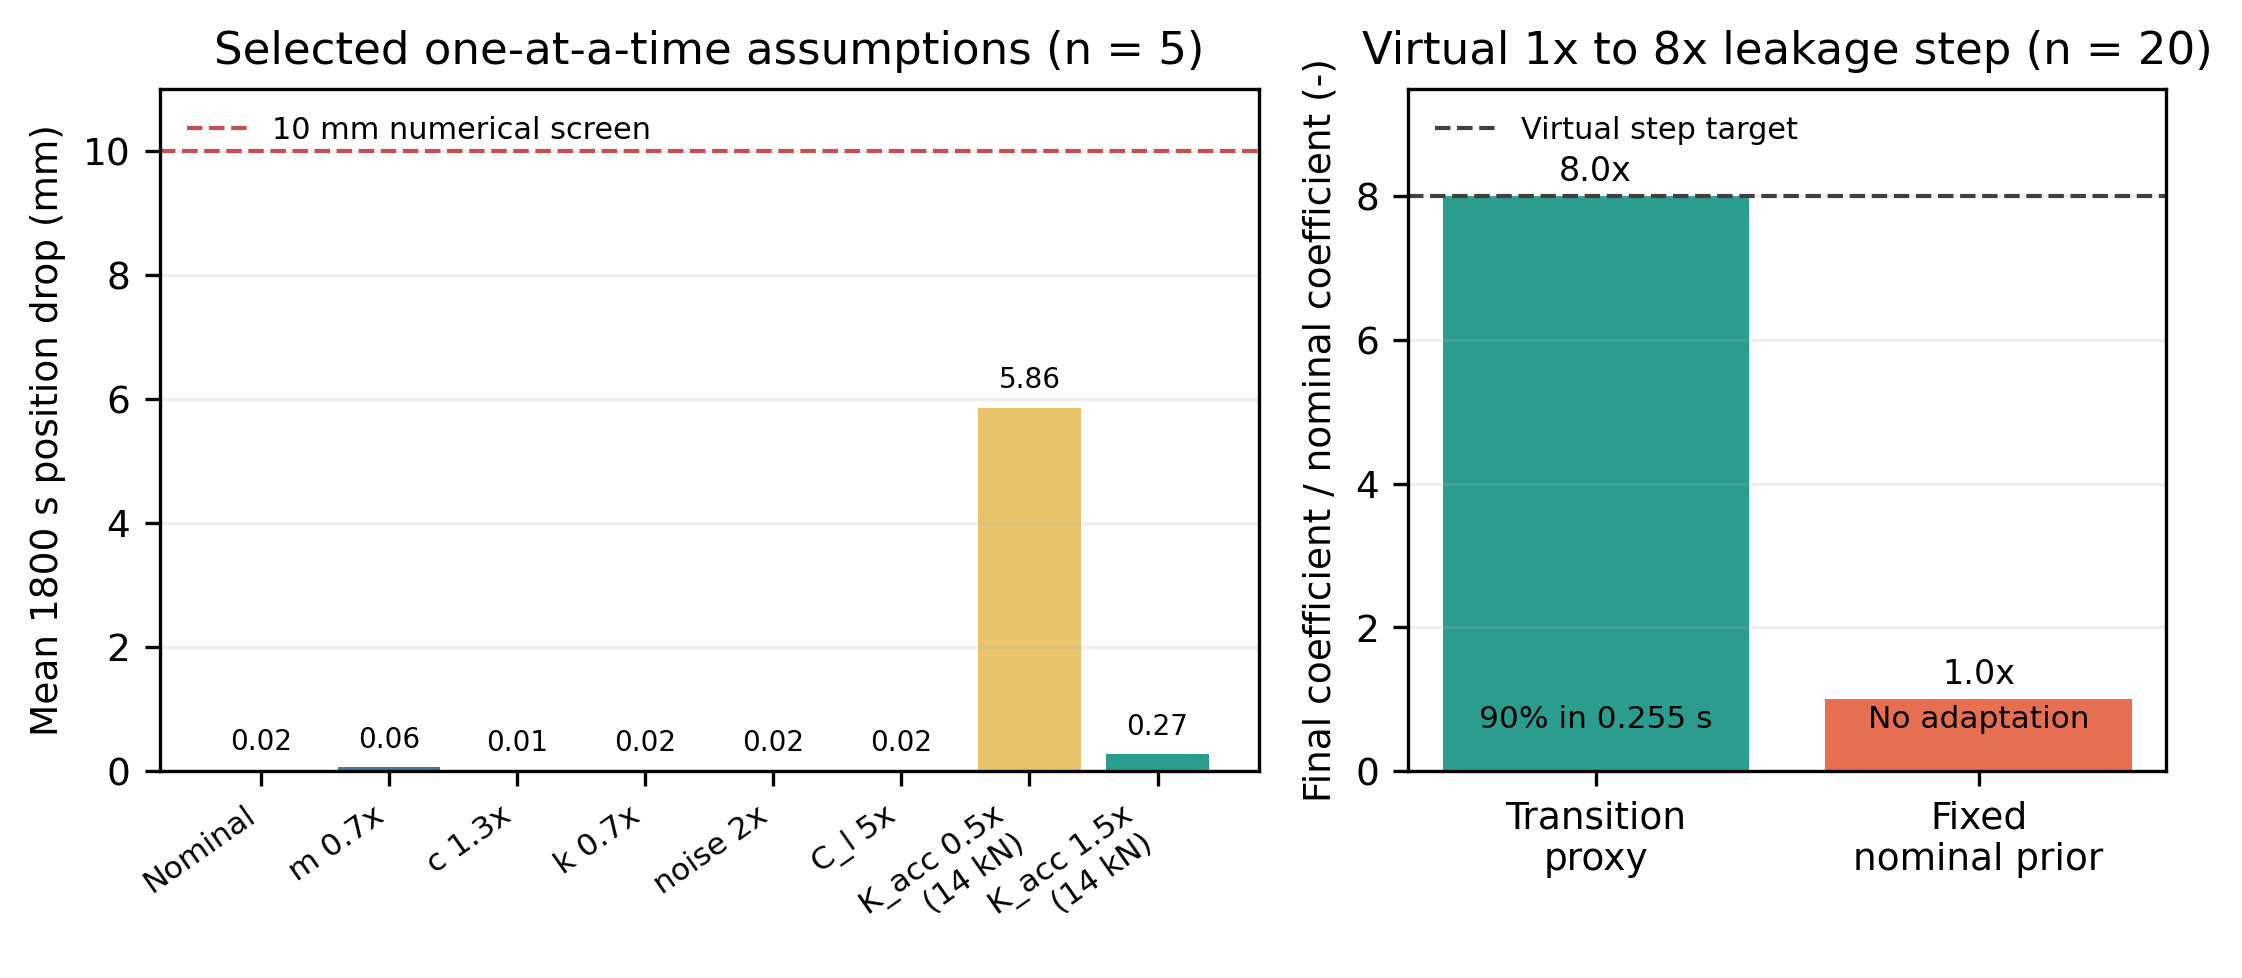
\includegraphics[width=0.94\linewidth]{paper1_assumption_and_proxy_stress.png}
\caption{Selected assumption-range screen (left, $n=5$) and virtual one-to-eight-times leakage step (right, $n=20$). Both panels are parameterized model tests, not calibrated-hitch evidence.}
\label{fig:assumption-proxy}
\end{figure}

\subsection{Temperature-load envelope and raw-velocity threshold}
The controller was next evaluated over a parameterized temperature-load envelope: constant oil temperatures of 25, 40, and 50 $^\circ$C were crossed with post-step loads of 7, 10, and 14 kN ($n=20$ per case). The filtered 3 mm s$^{-1}$ velocity gate entered hold in all nine cases. Figure~\ref{fig:envelope} shows that the highest mean 1800 s position drop was 1.93 mm (95\% CI: 1.74--2.11 mm) at 50 $^\circ$C and 14 kN. The result broadens the declared virtual operating envelope; its leakage and thermal inputs define internal model conditions rather than a physical temperature or load validation.

The same protocol was also evaluated with an unfiltered velocity signal. At raw thresholds of 3 and 5 mm s$^{-1}$, none of the 20 runs entered hold. Relaxing the raw threshold to 10 mm s$^{-1}$ produced 20/20 entries and a 0.031 mm mean drop (95\% CI: 0.016--0.047 mm). This sensitivity result identifies a candidate signal-processing design trade-off; it does not validate the original 3 mm s$^{-1}$ requirement or establish an acceptable hardware safety threshold.

\subsection{Transition-separated accuracy audit}
Because the commanded motion spans 200 mm, the all-time RMSE is dominated by the planned transition and is not a steady-state precision metric. We therefore recomputed accuracy after the 8 s reference transition. In the nominal virtual condition, the 20-seed mean post-transition RMSE was 4.25 mm, the mean 95th-percentile absolute error was 4.53 mm, and the mean per-seed maximum absolute error was 9.54 mm; the worst seed reached 10.61 mm. Doubling the position-noise standard deviation gave a mean maximum absolute error of 8.89 mm and a worst seed of 11.62 mm. These values support a statistical virtual accuracy description, but not a universal hard $\pm10$ mm guarantee.

\begin{figure}[H]
\centering
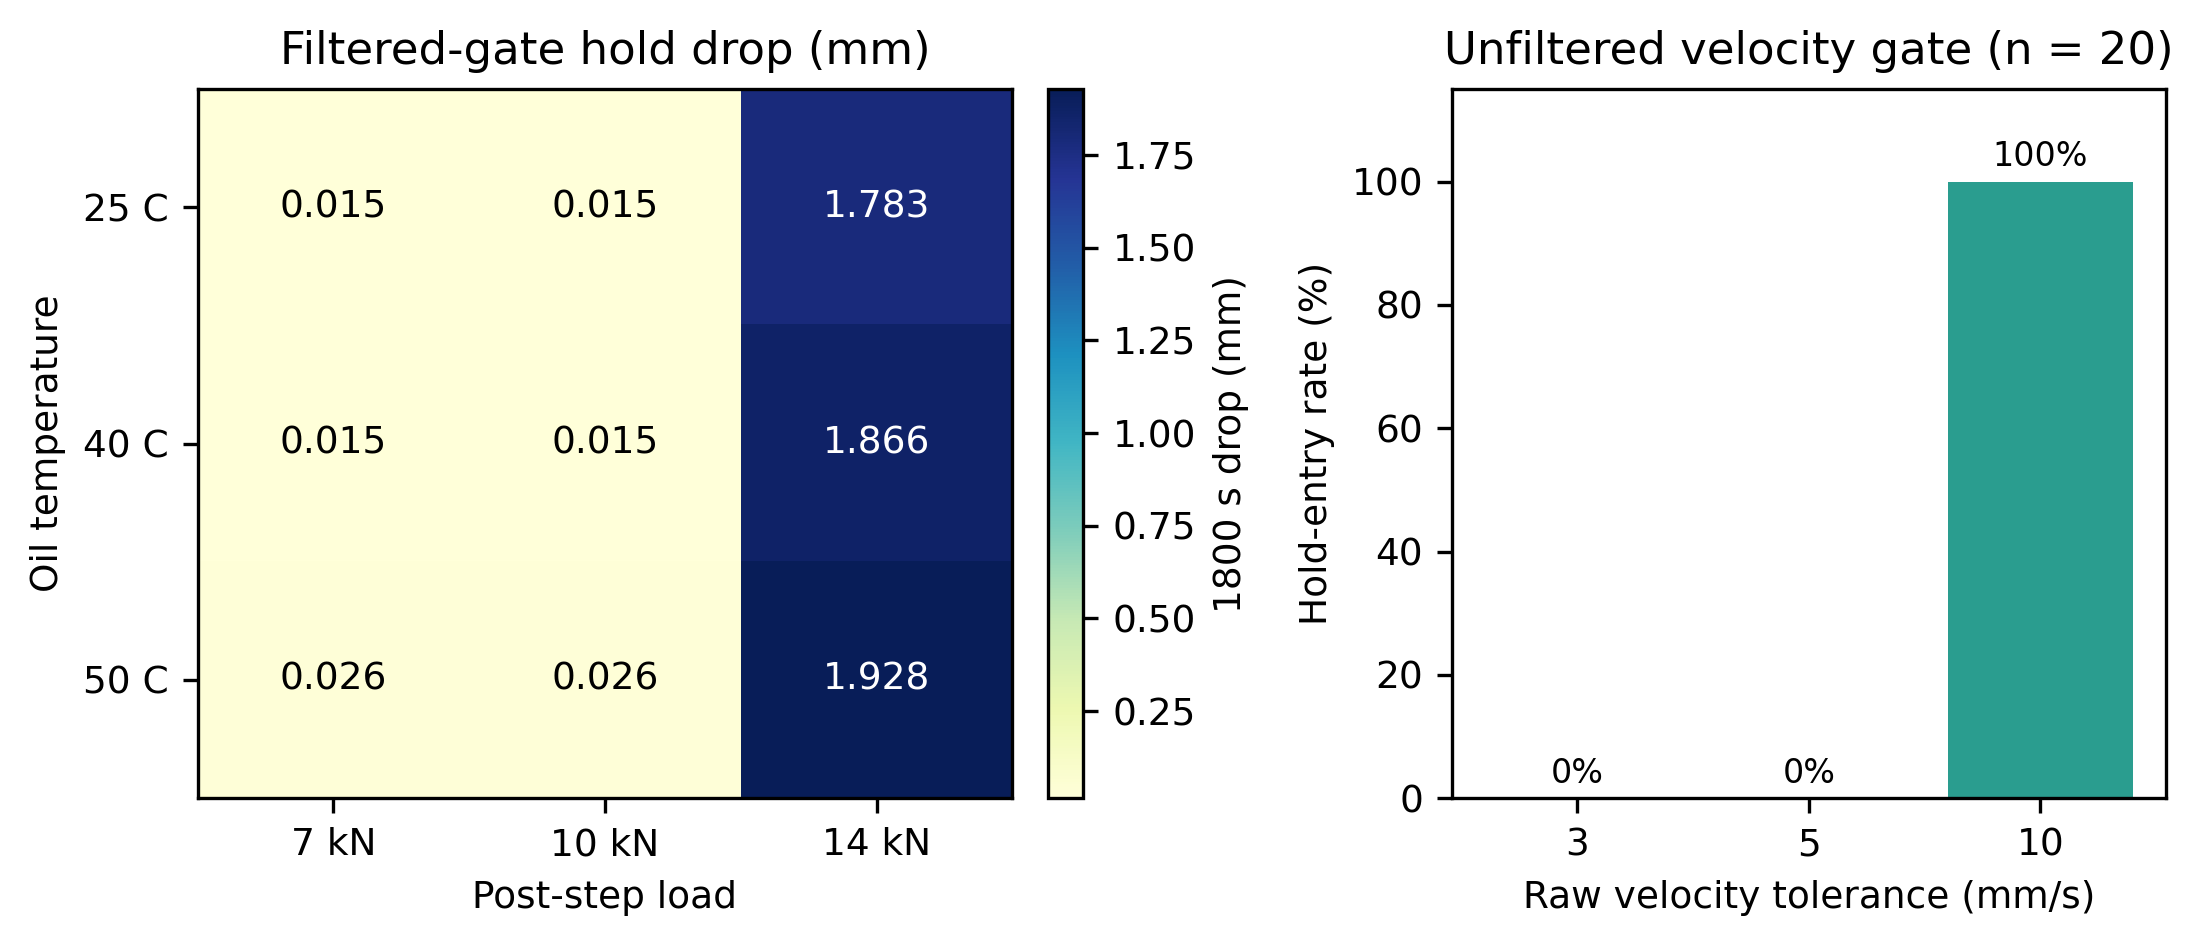
\includegraphics[width=0.94\linewidth]{paper1_operating_envelope.png}
\caption{Parameterized temperature-load envelope under the filtered velocity gate (left), and sensitivity of the unfiltered velocity gate to its tolerance (right), $n=20$ per condition.}
\label{fig:envelope}
\end{figure}

\subsection{Cartesian virtual stress surface}
To test interactions that are not visible in one-at-a-time screens, we evaluated the complete controller on a predeclared Cartesian surface crossing mass (0.7 and 1.3 times nominal), cylinder leakage (1 and 5 times nominal), constant temperature (25 and 50 $^\circ$C), post-step load (7 and 14 kN), and accumulator-flow coefficient (0.5 and 1.0 times nominal). The 32 cases used the same 20 noise seeds as the primary experiment, but no case was selected for tuning. All 640 runs entered hold and passed the 10 mm, 1800 s screen. The worst case was the combination of 0.7$\times$ mass, 1$\times$ leakage, 50 $^\circ$C, 14 kN, and 0.5$\times$ accumulator flow, with a mean drop of 7.99 mm (95\% CI: 7.77--8.21 mm). Figure~\ref{fig:combined-stress} is a deterministic virtual coverage surface, not a probability statement about physical machines.

\begin{figure}[H]
\centering
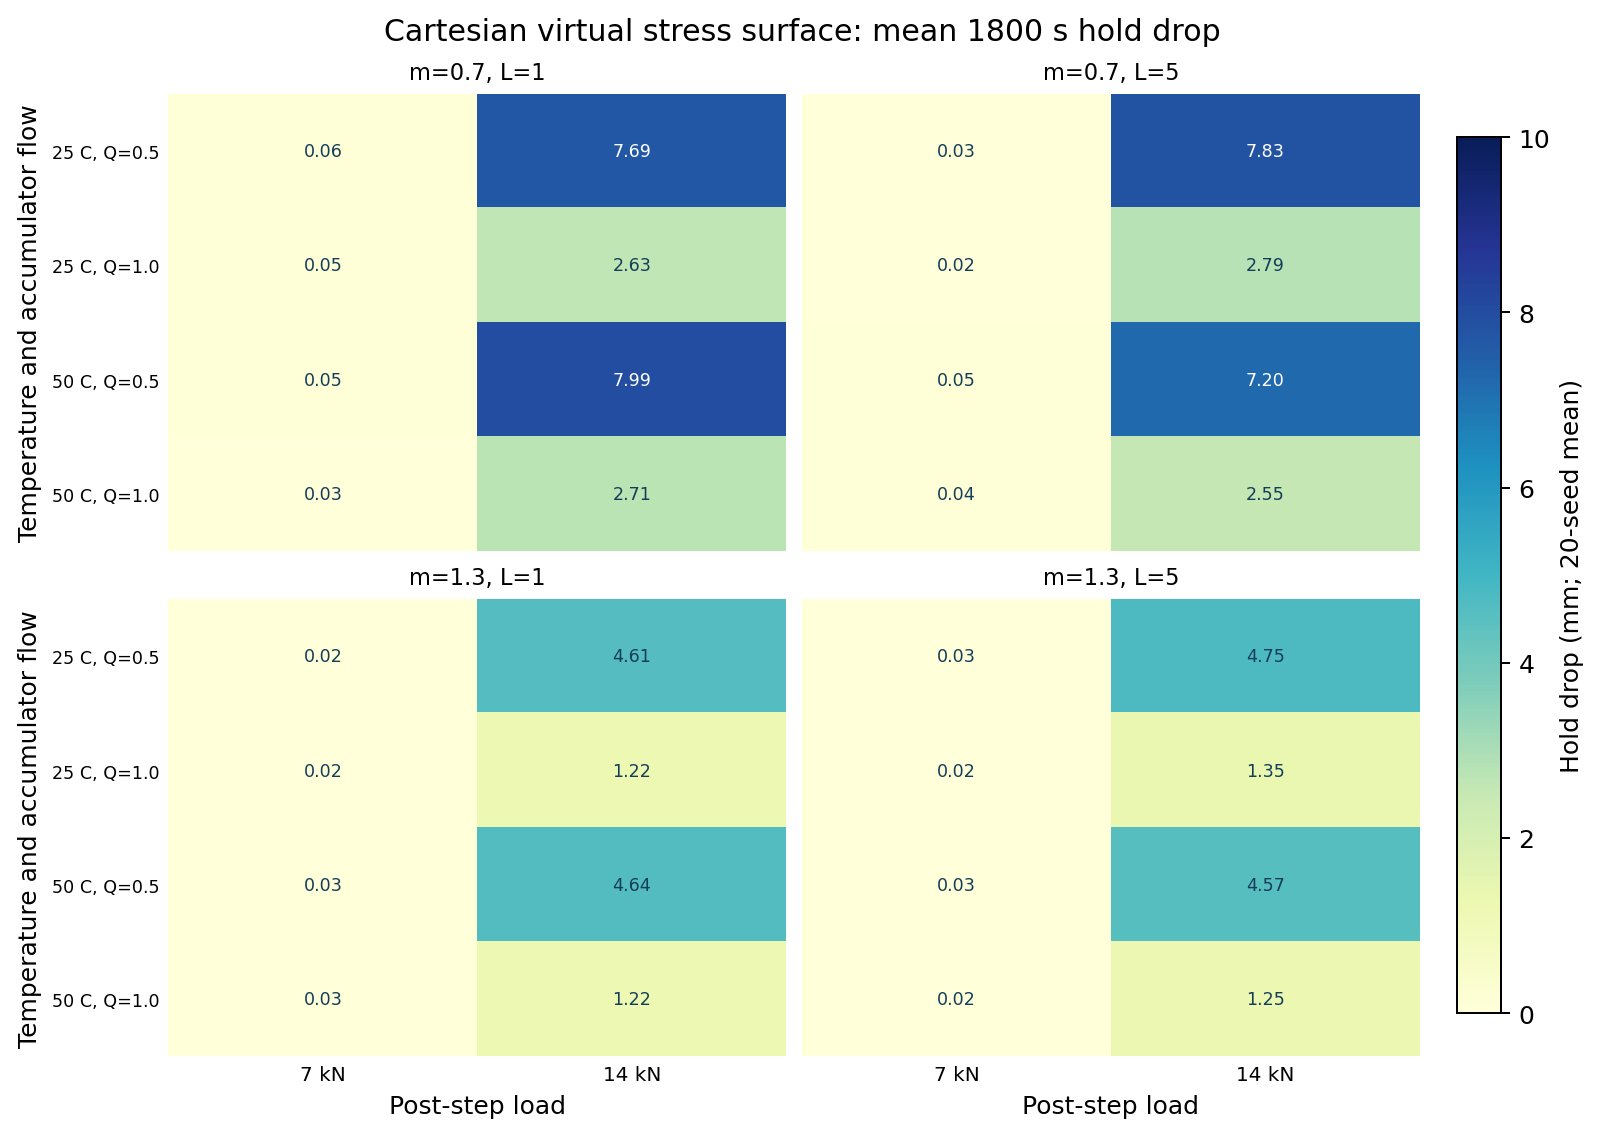
\includegraphics[width=0.99\linewidth]{paper1_combined_stress_surface.png}
\caption{Predeclared Cartesian virtual stress surface for the complete hitch controller. Each cell summarizes 20 seeds. Panels fix mass ($m$) and leakage multiplier ($L$); rows combine temperature ($T$) and accumulator-flow multiplier ($Q$), and columns show the post-step load. The color scale is fixed at 0--10 mm, and every cell passes the 10 mm screen.}
\label{fig:combined-stress}
\end{figure}

\subsection{Measurement-interface and observer-mismatch audit}
The nominal pressure signal in the primary protocol is a virtual interface, so a separate 20-seed audit (seeds 2060--2079) changed controller-facing measurements and observer coefficients while keeping the plant fixed. A $+2$ mm position bias retained hold entry but raised the worst steady error to 12.67 mm. More importantly, unfiltered 0.1 MPa Gaussian pressure noise caused post-entry instability: every run entered hold before its steady error reached the 500 mm virtual-stroke boundary. This failure is retained in Table~\ref{tab:measurement-audit}; it is not counted as a successful hold merely because entry occurred.

A declared 200 ms first-order pressure filter provided a restricted mitigation test. With 0.05 MPa pressure noise, all 20 runs entered hold and the worst steady error was 9.72 mm. The combined filtered case adds a $+2$ mm position bias, $+0.1$ MPa pressure bias, 0.05 MPa pressure noise, a $+0.5$ kN load-measurement bias, and conservative observer gain/rate mismatches; it entered hold in all 20 runs with an 8.97 mm worst steady error. These results define an interface-specific virtual boundary. They neither identify a hardware sensor budget nor convert the nominal result into a universal $\pm10$ mm guarantee.

\begin{table}[H]
\centering
\caption{Independent controller-facing measurement and observer audit ($n=20$ per row). All plant parameters remain fixed virtual inputs. The raw-noise row is an intentional retained failure boundary.}
\label{tab:measurement-audit}
\scriptsize
\setlength{\tabcolsep}{3pt}
\begin{tabularx}{\linewidth}{@{}X r r r r@{}}
\toprule
Case & Hold entry & Steady RMSE (mm) & Mean P95 abs. error (mm) & Worst steady error (mm) \\
\midrule
Nominal interface & 20/20 & 4.24 & 4.63 & 10.56 \\
$+2$ mm position bias & 20/20 & 4.25 & 4.63 & 12.67 \\
0.10 MPa raw pressure noise & 20/20 then unstable & 486.56 & 500.00 & 500.00 \\
0.05 MPa pressure noise, 200 ms filter & 20/20 & 4.69 & 5.55 & 9.72 \\
Combined filtered mismatch & 20/20 & 2.50 & 2.90 & 8.97 \\
\bottomrule
\end{tabularx}
\end{table}

\section{Discussion}
The simulation does not support a claim that the hybrid law has intrinsically better nominal tracking than PID or DI-SMAC. Its differentiated value is an explicit holding architecture and its behavior in the load-step and temperature-load tests. The 14 kN ablation supports the modeled load-feedforward and accumulator branches. By contrast, the fixed-prior and leakage-proxy runs had identical hold drops in the leakage-step screen. The proxy should therefore be interpreted as a transparent model-state and supervisory-mode diagnostic, not as evidence of a general observer-performance benefit.

The central modelling choices are the declared leakage paths, accumulator properties, friction, load measurement, and virtual pressure interface. The 20 repetitions perturb position-sensor noise and the 32-case surface tests deterministic parameter interactions; neither is a probability distribution or a physical-machine trial. The pressure-transition proxy is deliberately evaluated against the same virtual model that produces its state transition, so its rapid response is an internal-consistency result. The independent audit makes the observability boundary sharper: the raw 0.1 MPa pressure-noise case is unstable, whereas the explicitly filtered 0.05 MPa and combined mismatch cases remain bounded only within the stated virtual interface. The raw-velocity hold gate likewise remains a signal-processing design boundary: the 10 mm s$^{-1}$ result is a relaxed virtual setting, not a replacement safety criterion.

A separate fine-trim scan tested whether the load-step result was an artifact of the post-transition gain choice. Increasing the fine-trim gains by 1.5 times reduced the mean 14 kN hold drop from 1.75 to 0.73 mm, but increased the nominal mean maximum post-transition error from 9.54 to 9.92 mm and its worst seed to 11.60 mm. The 2-times setting reduced the 14 kN mean drop to 0.29 mm but produced a 13.04 mm nominal worst seed. The reported controller therefore retains the baseline gains and reports this trade-off rather than selecting a gain solely for the load-step metric.

The measurement audit is not used to select gains or censor unfavorable outcomes. It instead shows what must be true of a future sensing implementation before the nominal virtual architecture can be transferred: a raw pressure-noise interface at the tested 0.1 MPa level is not admissible, while the declared filtered 0.05 MPa interface is a bounded virtual condition. This preserves the distinction between an architecture-level stress test and physical validation, while making the controller's information assumptions inspectable.

\section{Conclusions}
This study presents a reproducible dual-mode hitch-control virtual prototype that combines pressure feedforward, a model-level leakage proxy, a hysteretic hold supervisor, accumulator compensation, and load feedforward. Under the declared parameterization, the complete controller meets the numerical position-holding screen, attenuates a 14 kN load-step disturbance, remains within 1.93 mm mean drop in the one-at-a-time temperature-load envelope, and passes all 640 runs of the Cartesian virtual stress surface, whose worst mean drop is 7.99 mm. The transition-separated audit gives a 4.25 mm nominal post-transition RMSE, but the worst seeded maximum error is 10.61 mm; therefore, the result is a statistical virtual accuracy characterization rather than a universal hard $\pm10$ mm guarantee. The original strict raw-velocity gate never entered hold; only a relaxed 10 mm s$^{-1}$ raw threshold entered all virtual runs. The independent measurement audit further retains an unfiltered 0.1 MPa pressure-noise instability and bounds a declared filtered combined mismatch to an 8.97 mm worst steady error. The contribution is a parameterized theoretical method and reproducible stress-test workflow; the reported boundaries belong to the declared virtual model and do not require real-machine calibration for their internal validity.

\authorcontributions{Conceptualization, C.C.; Methodology, C.C.; Software, C.C.; Formal analysis, C.C.; Visualization, C.C.; Writing---original draft preparation, C.C.; Resources, C.C.; Validation, P.W.; Investigation, C.C.; Writing---review and editing, Y.Z.; Supervision, Y.Z.; Project administration, Y.Z.; Funding acquisition, Y.Z.}
\funding{This work has received funding from the Science and Technology Project of the Ministry of Agriculture and Rural Affairs of China.}
\institutionalreview{Not applicable.}
\informedconsent{Not applicable.}
\dataavailability{The virtual-prototype source code, reproduction scripts, machine-readable parameter manifest, assumption register, traceability exporter, and JSON outputs supporting these results are publicly available at \url{https://github.com/Fat-pig-Cui/agricultural-tractor-virtual-prototypes}. The versioned Zenodo archive is accessible through the concept DOI \url{https://doi.org/10.5281/zenodo.22754509}, which resolves to the latest published archive version.}
\conflictsofinterest{The authors declare no conflicts of interest.}

\begin{thebibliography}{9}
\bibitem{sun2022} Sun, X.; Lu, Z.; Song, Y.; Cheng, Z.; Jiang, C.; Qian, J.; Lu, Y. Development Status and Research Progress of a Tractor Electro-Hydraulic Hitch System. \emph{Agriculture} \textbf{2022}, \emph{12}, 1547. \url{https://doi.org/10.3390/agriculture12101547}.
\bibitem{kumar2021} Kumar, S.; Tewari, V.K.; Bharti, C.K.; Ranjan, A. Modeling, simulation and experimental validation of flow rate of electro-hydraulic hitch control valve of agricultural tractor. \emph{Flow Measurement and Instrumentation} \textbf{2021}, \emph{82}, 102070. \url{https://doi.org/10.1016/j.flowmeasinst.2021.102070}.
\bibitem{sun2025} Sun, X.; Song, Y.; Lu, Z.; Deng, X. Research on a Coordinated Control Method of Tractor Electro-Hydraulic Hitch Tillage Depth and Travel Speed Based on Optimal Overall Efficiency and Economic Performance. \emph{Agriculture} \textbf{2025}, \emph{15}, 2232. \url{https://doi.org/10.3390/agriculture15212232}.
\bibitem{kim2025} Kim, E.-K.; Han, T.-H.; Lee, J.-H.; Han, C.-W.; Lim, R.-G. Tracking accuracy evaluation of autonomous agricultural tractors via rear three-point hitch estimation using a hybrid model of EKF-Transformer. \emph{Agriculture} \textbf{2025}, \emph{15}, 1475. \url{https://doi.org/10.3390/agriculture15141475}.
\bibitem{liu2023} Liu, C.; Gu, J.; Du, X.; Liu, C.; Du, Y.; Mao, E. Differential and integral sliding mode adaptive control algorithm for draft and position integrated control of electro-hydraulic hitch in agricultural tractor. \emph{INMATEH Agricultural Engineering} \textbf{2023}, \emph{70}, 369--378. \url{https://doi.org/10.35633/inmateh-70-36}.
\bibitem{bai2010} Bai, Y.; Li, P. Adaptive fuzzy sliding mode control for electro-hydraulic position servo system. \emph{2010 Chinese Control and Decision Conference} 2010, 3249--3253. \url{https://doi.org/10.1109/CCDC.2010.5498613}.
\bibitem{tang2011} Tang, R.; Zhang, Q. Dynamic sliding mode control scheme for electro-hydraulic position servo system. \emph{Procedia Engineering} \textbf{2011}, \emph{24}, 28--32. \url{https://doi.org/10.1016/j.proeng.2011.11.2596}.
\bibitem{jin2013} Jin, B. Chattering inhibition of variable rate reaching law sliding mode control for electro-hydraulic position servo system. \emph{Journal of Mechanical Engineering} \textbf{2013}, \emph{49}, 163--169. \url{https://doi.org/10.3901/JME.2013.10.163}.
\bibitem{jelali2003} Jelali, M.; Kroll, A. \emph{Hydraulic Servo-systems: Modelling, Identification and Control}; Springer: London, UK, 2003. \url{https://doi.org/10.1007/978-1-4471-0099-7}.
\end{thebibliography}
\end{document}
